% !TEX program = xetex
% !TEX encoding = UTF-8 Unicode

\PassOptionsToPackage{usenames,dvipsnames}{xcolor}
\PassOptionsToPackage{colorlinks,linktoc=all}{hyperref}
% \documentclass[sigconf, anonymous, review]{acmart} % for review
\documentclass[sigconf]{acmart} % for arxiv
\settopmatter{authorsperrow=4}

%%
%% \BibTeX command to typeset BibTeX logo in the docs
\AtBeginDocument{%
  \providecommand\BibTeX{{%
    \normalfont B\kern-0.5em{\scshape i\kern-0.25em b}\kern-0.8em\TeX}}}

%% Rights management information.  This information is sent to you
%% when you complete the rights form.  These commands have SAMPLE
%% values in them; it is your responsibility as an author to replace
%% the commands and values with those provided to you when you
%% complete the rights form.
\setcopyright{acmcopyright}
\copyrightyear{2018}
\acmYear{2018}
\acmDOI{10.1145/1122445.1122456}

%% These commands are for a PROCEEDINGS abstract or paper.
\acmConference[KDD 2020]{}{August 23–27, 2020}{}
\acmBooktitle{KDD '20: International Workshop on Industrial Recommendation Systems, August 23--27, 2020}
\acmPrice{15.00}
\acmISBN{978-1-4503-XXXX-X/18/06}

%%
%% Submission ID.
%% Use this when submitting an article to a sponsored event. You'll
%% receive a unique submission ID from the organizers
%% of the event, and this ID should be used as the parameter to this command.
%%\acmSubmissionID{123-A56-BU3}

%%
%% The majority of ACM publications use numbered citations and
%% references.  The command \citestyle{authoryear} switches to the
%% "author year" style.
%%
%% If you are preparing content for an event
%% sponsored by ACM SIGGRAPH, you must use the "author year" style of
%% citations and references.
%% Uncommenting
%% the next command will enable that style.
%%\citestyle{acmauthoryear}

% !TEX root = ../recommending-interesting-writing.tex

% FONTS
%\usepackage[T1]{fontenc}

% Replace default Latin Modern typewriter with its proportional counterpart
% http://www.tug.dk/FontCatalogue/lmoderntypewriterprop/
%\renewcommand*\ttdefault{lmvtt}

%%% OPTION 3 - MTPRO 2 Math + Termes Times + ParaType Sans
\let\myBbbk\Bbbk
\let\Bbbk\relax
%\usepackage{tgtermes}
\usepackage{amsmath}
% \usepackage[subscriptcorrection,
%             amssymbols,
%             mtpbb,
%             mtpcal,
%             nofontinfo  % suppresses all warnings
%            ]{mtpro2}
% \usepackage{scalefnt,letltxmacro}
% \LetLtxMacro{\oldtextsc}{\textsc}
% \renewcommand{\textsc}[1]{\oldtextsc{\scalefont{1.10}#1}}
% \usepackage[scaled=0.92]{PTSans}

% ICONS
\usepackage{fontawesome}

% CODE
\usepackage{minted}

% COLOR
%\usepackage[usenames,dvipsnames]{xcolor}
\definecolor{shadecolor}{gray}{0.9}

% SPACING and TEXT
%\usepackage[final,expansion=alltext]{microtype}
%\usepackage[english]{babel}
\usepackage[parfill]{parskip}
\usepackage{afterpage}
\usepackage{framed}
\usepackage{nicefrac}

% EDITING
% line numbering in left margin
\usepackage{lineno}
\renewcommand\linenumberfont{\normalfont
                             \footnotesize
                             \sffamily
                             \color{SkyBlue}}
% ragged paragraphs in right margin
\usepackage{ragged2e}
\DeclareRobustCommand{\sidenote}[1]{\marginpar{
                                    \RaggedRight
                                    \textcolor{Plum}{\textsf{#1}}}}

% Define a paragraph header function
\DeclareRobustCommand{\parhead}[1]{\textbf{#1}~}

% paragraph helper
\DeclareRobustCommand{\PP}{\textcolor{Plum}{\P}~}
\DeclareRobustCommand{\pp}{\textcolor{Plum}{\P}~}

% COUNTERS
\renewcommand{\labelenumi}{\color{black!67}{\arabic{enumi}.}}
\renewcommand{\labelenumii}{{\color{black!67}(\alph{enumii})}}
\renewcommand{\labelitemi}{{\color{black!67}\textbullet}}

% FIGURES
\usepackage{graphicx}
\usepackage[labelfont=bf]{caption}
\usepackage[format=hang]{subcaption}

% TABLES
\usepackage{booktabs}
%\usepackage{dblfloatfix}  % for placing table at bottom of page

% TABLE ALIGNMENT
\usepackage{etoolbox,siunitx}
\robustify\bfseries
\sisetup{detect-weight=true, detect-shape=true, detect-mode=true,
table-format=5.1,
table-number-alignment=center,
separate-uncertainty=true,
input-ignore={,},input-decimal-markers={.}}

% BABEL
% \usepackage{polyglossia}

% BIBLIOGRAPHY
%\usepackage[backend=biber, style=numeric-comp, isbn=false, issn=false, doi=false]{biblatex}
\usepackage{natbib}

% ALGORITHMS
\usepackage[algoruled]{algorithm2e}
\usepackage{listings}
\usepackage{fancyvrb}
\fvset{fontsize=\normalsize}

% THEOREMS
\usepackage{amsthm}
\newtheorem{theorem}{Theorem}
% \newtheorem{proposition}[proposition]{Proposition}
\newtheorem{prop}{Proposition}


% TODO
\usepackage{todo}

% HYPERREF
%\usepackage[colorlinks,linktoc=all]{hyperref}
\usepackage[all]{hypcap}
\hypersetup{citecolor=Violet}
\hypersetup{linkcolor=black}
\hypersetup{urlcolor=MidnightBlue}

% CLEVEREF must come after HYPERREF
\usepackage[capitalize]{cleveref}

% ACRONYMS
\usepackage[acronym,smallcaps,nowarn]{glossaries}
% \makeglossaries

% COLOR DEFINITIONS
\newcommand{\red}[1]{\textcolor{BrickRed}{#1}}
\newcommand{\orange}[1]{\textcolor{BurntOrange}{#1}}
\newcommand{\green}[1]{\textcolor{OliveGreen}{#1}}
\newcommand{\blue}[1]{\textcolor{MidnightBlue}{#1}}
\newcommand{\gray}[1]{\textcolor{black!60}{#1}}

% LISTINGS DEFINTIONS
\usepackage{listings}
\lstdefinestyle{alp_style}{
    commentstyle=\color{OliveGreen},
    numberstyle=\tiny\color{black!60},
    stringstyle=\color{BrickRed},
    basicstyle=\ttfamily\scriptsize,
    breakatwhitespace=false,
    breaklines=true,
    captionpos=b,
    keepspaces=true,
    numbers=none,
    numbersep=5pt,
    showspaces=false,
    showstringspaces=false,
    showtabs=false,
    tabsize=2
}
\lstset{style=alp_style}

% !TEX root = ../set_recommendation.tex

\DeclareRobustCommand{\mb}[1]{\ensuremath{\boldsymbol{\mathbf{#1}}}}
%\DeclareRobustCommand{\mb}[1]{\mathbold{#1}}

\DeclareRobustCommand{\KL}[2]{\ensuremath{\textrm{KL}\left(#1\;\|\;#2\right)}}

\DeclareMathOperator*{\argmax}{arg\,max}
\DeclareMathOperator*{\argmin}{arg\,min}

\newcommand{\yum}{y_{um}}
\newcommand{\xum}{x_{um}}
\newcommand{\xuk}{x_{uk}}
\newcommand{\yuk}{y_{uk}}
\renewcommand{\mid}{~\vert~}
\newcommand{\prm}{\:;\:}

\newcommand{\mbw}{\mb{w}}
\newcommand{\mbW}{\mb{W}}

\newcommand{\mbx}{\mb{x}}
\newcommand{\mbX}{\mb{X}}

\newcommand{\mby}{\mb{y}}
\newcommand{\mbY}{\mb{Y}}

\newcommand{\mbz}{\mb{z}}
\newcommand{\mbZ}{\mb{Z}}

\newcommand{\mbI}{\mb{I}}
\newcommand{\mbone}{\mb{1}}

\newcommand{\mbL}{\mb{L}}

\newcommand{\mbtheta}{\mb{\theta}}
\newcommand{\mbTheta}{\mb{\Theta}}
\newcommand{\mbomega}{\mb{\omega}}
\newcommand{\mbOmega}{\mb{\Omega}}
\newcommand{\mbsigma}{\mb{\sigma}}
\newcommand{\mbSigma}{\mb{\Sigma}}
\newcommand{\mbphi}{\mb{\phi}}
\newcommand{\mbPhi}{\mb{\Phi}}

\newcommand{\mbalpha}{\mb{\alpha}}
\newcommand{\mbbeta}{\mb{\beta}}
\newcommand{\mbgamma}{\mb{\gamma}}
\newcommand{\mbeta}{\mb{\eta}}
\newcommand{\mbmu}{\mb{\mu}}
\newcommand{\mbrho}{\mb{\rho}}
\newcommand{\mblambda}{\mb{\lambda}}
\newcommand{\mbzeta}{\mb{\zeta}}

\newcommand\dif{\mathop{}\!\mathrm{d}}
\newcommand{\diag}{\textrm{diag}}
\newcommand{\supp}{\textrm{supp}}

\newcommand{\E}{\mathbb{E}}
\newcommand{\V}{\mathbb{V}}
\newcommand{\bbH}{\mathbb{H}}

\newcommand{\bbN}{\mathbb{N}}
\newcommand{\bbZ}{\mathbb{Z}}
\newcommand{\bbR}{\mathbb{R}}
\newcommand{\bbS}{\mathbb{S}}

\newcommand{\cL}{\mathcal{L}}
\newcommand{\cS}{\mathcal{S}}
\newcommand{\cD}{\mathcal{D}}

\newcommand{\cN}{\mathcal{N}}
\newcommand{\cT}{\mathcal{T}}

\newcommand{\mult}{\textrm{Mult}}
\newcommand{\dirichlet}{\textrm{Dirichlet}}
\newcommand{\Gam}{\textrm{Gamma}}
\newcommand{\Pois}{\textrm{Poisson}}
% !TEX root = set_recommendation.tex

\newacronym{ELBO}{elbo}{evidence lower bound}
\newacronym{GMM}{gmm}{Gaussian mixture model}
\newacronym{KL}{kl}{Kullback-Leibler}
\newacronym{LDA}{lda}{latent Dirichlet allocation}
\newacronym{SVI}{svi}{stochastic variational inference}
\newacronym{DEF}{def}{deep exponential family}
\newacronym{rfs}{rfs}{\textsc{rankfromsets}}
\newacronym{ctpf}{ctpf}{collaborative topic Poisson factorization}

\title{Recommending Interesting Writing}
% keywords:
% deep learning
% collaborative filtering
% negative sampling
% content-based recommendation
% food recommender systems
% \begin{framed}
% \centering
% \textsc{do not cite or redistribute.}
% \end{framed}

\author{Rohan Bansal}
\affiliation{\institution{The Browser}}
\email{rohan@thebrowser.com}

\author{Uri Bram}
\affiliation{\institution{The Browser}}
\email{uri@thebrowser.com}

\author{Robert Cottrell}
\affiliation{\institution{The Browser}}
\email{robert@thebrowser.com}

\author{Jaan Altosaar}
\orcid{0000-0003-1294-4159}
\affiliation{\institution{Princeton University}}
\email{altosaar@princeton.edu}

%%
%% By default, the full list of authors will be used in the page
%% headers. Often, this list is too long, and will overlap
%% other information printed in the page headers. This command allows
%% the author to define a more concise list
%% of authors' names for this purpose.
\renewcommand{\shortauthors}{Trovato and Tobin, et al.}

\begin{document}
% !TEX root = recommending-interesting-writing.tex
\begin{abstract}
  We describe a system for recommending nonfiction writing to editors at The Browser, a curation service for interesting writing. The editors' goal is select articles from a large list of candidates, and these selections of nonfiction writing are shared with subscribers. To aid the editors, we build a recommender system that classifies articles based on their content. The recommendation model is \gls{rfs}, chosen for its scalability and explainability, with architectures that allow editors to understand which words in an article informed a recommendation~\citep{altosaar2020rankfromsets:}. Further, editors can choose which latent features of articles to upweight. We train \gls{rfs} on historical data, and show that this translates to good performance in an online setting with qualitative feedback from editors on unseen candidate articles. Due to resource constraints, we deploy \gls{rfs} using a microservices architecture on a cloud computing platform. For reproducibility and transparency of the user-facing system, we open source the end-to-end pipeline and release a demo\footnote{\url{https://the-browser.github.io/recommending-interesting-writing/}}, data collection, training and deployment scripts, and model parameters.\footnote{\url{https://github.com/the-browser/recommending-interesting-writing}}
\end{abstract}
%%
%% The code below is generated by the tool at http://dl.acm.org/ccs.cfm.
%% Please copy and paste the code instead of the example below.
%%
\begin{CCSXML}
<ccs2012>
   <concept>
       <concept_id>10010405.10010497.10010498</concept_id>
       <concept_desc>Applied computing~Document searching</concept_desc>
       <concept_significance>500</concept_significance>
       </concept>
   <concept>
       <concept_id>10010147.10010257.10010282.10010292</concept_id>
       <concept_desc>Computing methodologies~Learning from implicit feedback</concept_desc>
       <concept_significance>500</concept_significance>
       </concept>
 </ccs2012>
\end{CCSXML}

\ccsdesc[500]{Applied computing~Document searching}
\ccsdesc[500]{Computing methodologies~Learning from implicit feedback}

%%
%% Keywords. The author(s) should pick words that accurately describe
%% the work being presented. Separate the keywords with commas.
\keywords{content-based recommendation, open source, user interface}

%% A "teaser" image appears between the author and affiliation
%% information and the body of the document, and typically spans the
%% page.
\begin{teaserfigure}
  
\includegraphics[width=\textwidth]{fig/pipeline.pdf}
  \caption{\textbf{End-to-end pipeline for recommending nonfiction writing to editors at The Browser.} Positive examples for the \acrlong{rfs} recommendation model~\citep{altosaar2020rankfromsets:} are collected from editors' history of curated articles, and negative examples from news sources. After training and offline evaluation of the recommendation model, it is deployed as a microservice, and editors' feedback on the recommendation performance is used to inform refinement of data collection, training, and architectural choices in the recommendation model.}
  \Description{End-to-end pipeline for recommending nonfiction writing to editors at The Browser.}
  \label{fig:pipeline}
\end{teaserfigure}

%%
%% This command processes the author and affiliation and title
%% information and builds the first part of the formatted document.
\maketitle
% !TEX root = recommending-interesting-writing.tex
\section{Introduction}
\label{sec:introduction}
Creative nonfiction, longform journalism, and blog posts are examples of the types of articles curated by The Browser's team of editors. The editors read a large number of articles from various publications to select content to recommend to subscribers.

In building a recommender system to help editors sift through many documents, it is motivating to highlight the trade-off in user privacy intrinsic to recommender systems. A machine learning model must exploit information about a user. However, the incentive structures of operating a recommender system within a business can influence decisions around privacy and transparency~\citep{diakopoulos2020oxford}. For example, business models that rely on online advertising may engender recommender systems that upweight attention-grabbing content and hence time spent looking at ads. Such content might maximize a user's time spent with a service over time at the expense of long-term user experience or consent. In comparison, privacy-preserving and open source tools such as the Signal encrypted messaging service\footnote{\url{https://signal.org/}} may provide improved user experience in terms of privacy-preserving, transparent, and explainable algorithms and visual interfaces~\citep{cohn-gordon2017a-formal}. But the incentive structures for releasing recommender systems and visual interfaces that exploit private information about users are poor. There are few examples of end-to-end, open source, free-to-deploy pipelines for recommending content to users using a visual interface. This motivates building and deploying a recommendation model and corresponding explanation-aware visual interface to give users control, and inform them about how data is being used to make recommendations.

We build an end-to-end recommender system visual interface to address two aims: (1) to aid editors at The Browser in their decision-making task, and give them control through an explanation-aware interface, and (2) to release a lightweight, performant, open-source visual interface framework for explanation-aware recommender systems for document recommendation. In an offline evaluation, we show that the recommendation model we use for the visual interface outperforms \acrshort{bert}, a competitive document classification model. In a qualitative study, the control and explanations provided by the visual interface help editors in their decision-making and help find bugs in the recommendation model.
% % !TEX root = set_recommendation.tex
\section{Background}
\newcommand{\x}{\faCheck}
\begin{table*}%[!b]
  \begin{center}
    \begin{tabular}{lcccccc}
      \toprule
      Recommendation model & Uses attributes & Only user-item interactions & Scalable & Permutation-invariant & Loss tied to evaluation \\
      \midrule
      \acrlong{rfs} & \x & \x & \x & \x & \x \\
      \citet{wang2011collaborative} & \x & \x & & \x & \\
      \citet{gopalan2014content-based}& \x & \x  &  & \x &\\
%      \citet{lian2018towards} & & & \x & & \\
      \citet{dong2017a-hybrid}& \x & & & \x &\\
      \citet{chen2017joint}&\x & &\x & &\\
      \citet{bansal2016ask-the-gru:}&\x & \x & & &\\
      \citet{xu2017tag-aware}& \x & & \x & \x &\\
      \citet{rendle2009bpr:}&  & \x &  & & \x\\
      \citet{shi2012tfmap:} &\x & \x & & \x & \x\\
      \citet{wu2018starspace:} &\x & &\x &\x &\\
      \citet{kula2015metadata} & \x & \x &  & \x &\\
      \citet{shi2012climf:} & & \x & & &\x \\
      \citet{chen2018a-collective} & \x & \x & & \x & \\
      \citet{liu2014recommending} & \x & & & \x & \x \\
      \citet{cao2017embedding} & \x & &  & & \x \\
      \citet{okura2017embedding-based} & \x & & \x & & \x \\
%      \citet{zhang2018discrete} & \x & \x & \x & \x &\\
      \bottomrule
    \end{tabular}
    \caption{\label{tab:background}\acrlong{rfs} is a scalable recommendation
      model that recommends items using attributes, and is trained on an
      objective function connected to an evaluation metric. Most methods we
      highlight use attributes; some require data in addition to the user-item
      matrix of observations. Some models are invariant to permutation of the
      attributes, and may use a loss function that is connected to a
      recommendation performance metric. Few methods are scalable, as most
      recommendation models that use item side information require learning
      parameters for every item. }
    \vspace{-0.5cm}
  \end{center}
\end{table*}


%%% Local Variables:
%%% mode: latex
%%% TeX-master: "../set_recommendation"
%%% End:


We highlight two themes in research on recommendation models. We describe
recommendation models that incorporate side information and models that optimize
proxies of ranking metrics, and summarize this related work
in~\Cref{tab:background}.

\paragraph{Recommendation with side information} Side information is included in
recommendation models in several ways; we focus on deep learning and matrix
factorization approaches. Item side information can be modeled with deep
representations
\cite{zhang2017deep,bansal2016ask-the-gru:,lian2018towards,dong2017a-hybrid,chen2017joint,liang2018trsdl:,zuo2016tag-aware,xu2017tag-aware}
or can be included in content-based matrix factorization models as an additional
matrix
\cite{shi2014collaborative,gopalan2014content-based,wang2011collaborative,zhen2009tagicofi:,loepp2019interactive,bogers2018tag-based}.
Some deep learning based approaches scale to large datasets, but may not have
loss functions tied to evaluation metrics, or require data besides user-item
interactions. Content-based matrix factorization methods require learning
parameters for every item, and do not scale to data with large numbers of items.

\paragraph{Learning to rank} Recommendation models can be trained on loss
functions that approximate ranking-based evaluation metrics
\cite{yu2018walkranker:,liang2018top-n-rank:,rendle2009bpr:,song2018neural}, and
these models may include side information
\cite{shi2012tfmap:,yuan2016optimizing,ying2016collaborative,cao2017embedding,okura2017embedding-based}.
Such approaches may require data in addition to the user-item matrix, per-item
parameters, or use models where the output depends on the ordering of item
attributes.

%%% Local Variables:
%%% mode: latex
%%% TeX-master: "set_recommendation"
%%% End:

% as they are relevant to
% modeling items with attributes

% \paragraph{Deep representations of side information}
% Deep learning-based recommendation models incorporate side information in
% multiple ways \cite{zhang2017deep}. For example, items that have words as
% attributes can be represented using recurrent neural
% networks~\cite{bansal2016ask-the-gru:}. \citet{lian2018towards} use an attention
% mechanism to weight recommendations according to available item and user side
% information but not attributes, and \citet{dong2017a-hybrid} use denoising
% autoencoders to model side information in a deep recommendation model, but
% requires fitting parameters for every item. An example of a more efficient
% approach is the method in \citet{chen2017joint}, where embeddings are jointly
% learned for users, items, and item text for recommendation, but this method
% focuses on unsupervised pre-training of text representations. There are several
% examples of `tag-aware' or `tag-based' deep recommendation
% models~\cite{liang2018trsdl:,zuo2016tag-aware}, such as
% \citet{xu2017tag-awarey}, which focuses on data where users and items have
% different attributes and use autoencoders to learn user, item, and attribute
% representations. They use a cosine similarity-based objective function which is
% not tied to a metric used to evaluate recommendation performance.
%, but this method requires
%collecting information about which items users decided not to consume.

% \paragraph{Matrix factorization with side information}
% \citet{shi2014collaborative} survey several matrix factorization methods that
% incorporate side information. \citet{gopalan2014content-based} develop a
% Bayesian matrix factorization model for recommending items based on side
% information in the form of words in documents. \citet{wang2011collaborative}
% develop a regression model that uses a topic model to incorporate side
% information into recommendations. There are also several `tag-based' or
% `tag-aware' content-based matrix factorization
% models~\cite{zhen2009tagicofi:,loepp2019interactive,bogers2018tag-based}. Such
% content-based matrix factorization methods maximize the conditional
% log-likelihood of the data (or a bound on the log-likelihood); optimizing these
% objective functions does not optimize an evaluation metric. Furthermore, all of
% these methods are not scalable to large numbers of items as they require
% learning unique parameters for every item. Specifically, such content-based
% matrix factorization methods require learning a matrix that has a row for every
% item. For items with attributes, it is often infeasible to store this matrix in
% memory or exploit efficient coordinate ascent optimization schemes that require
% processing this entire matrix.

% \subsection{Recommendation via ranking}


% We describe recommendation models trained on
% such loss functions and extensions that include side information.

% \paragraph{Learning to rank}
% The literature on learning to rank includes models that optimize proxies of
% evaluation metrics, such as mean average precision, mean reciprocal rank, or
% discounted cumulative gain~\cite{yu2018walkranker:,liang2018top-n-rank:}. Forb
% example, Bayesian personalized ranking models optimize a pairwise ranking
% objective function \cite{rendle2009bpr:} that trains the model to rank items a
% user consumed higher than items a user did not consume. This objective is a
% heuristic motivated by an analogy to the receiver operating characteristic; a
% model trained on this objective does not provably maximize this metric. 
% \citet{song2018neural} extend Bayesian personalized ranking using deep neural
% networks, but do not model side information.

% \paragraph{Learning to rank with side information}
% Models that optimize proxies of ranking metrics that use side information
% include \citet{shi2012tfmap:}, where a smoothed approximation of mean average
% precision is used as a loss function. \citet{yuan2016optimizing} use a proxy of
% a ranking loss to fit a polynomial that models predictions of item consumption
% using item and side information features. \citet{ying2016collaborative} uses
% denoising autoencoders to represent item information in a model trained with a
% pairwise ranking loss. \citet{cao2017embedding} use a ranking loss to jointly
% learn embeddings of items and attributes; they focus on the case where users
% interact directly with both attributes and items with said attributes. All of
% these models require learning unique parameters for every item, and do not scale
% to large numbers of items. An example of a scalable method that uses the
% Bayesian personalized ranking criterion is in \citet{okura2017embedding-based},
% but this approach requires data with timestamps and negative item feedback.


% \paragraph{Order-invariant models.} Deep learning architectures have been
% developed for set-valued input. Such architectures are invariant to permutations
% of set elements and can approximate any order-invariant function
% \cite{zaheer2017deep,ravanbakhsh2017equivariance}. This work
% addresses regression whereas we focus on recommendation, and develop a negative
% sampling technique.
% %
% \citet{kumar2018representation} extend the order-invariant architectures to the
% problem of a set-valued response; we focus on set-valued input for which data is
% more readily available.
% %
% \citet{benson2018sequences} study the problem of predicting sets in a sequential
% order. The task is to predict attributes of a new item given the number of
% attributes. These attributes are modeled as coming from the attributes of the
% items a user has recently consumed. In contrast, we do not focus on temporal
% data and do not focus on repeated consumption of whole or partial copies of of
% items' sets of attributes.

% \paragraph{Ranking models.} Bayesian personalized ranking models optimize a
% ranking criterion \cite{rendle2009bpr:} that trains the model to rank items a
% user consumed higher than items a user did not consume. The criterion is
% motivated by an analogy to the receiver operating characteristic, but they do
% not prove that optimizing the criterion is equivalent to optimizing this metric.
% In our work, we prove (in \Cref{prop:maximizing-recall}) that our approach
% directly optimizes recall.
% %
% The Bayesian personalized ranking criterion has been extended to recommending
% news articles \cite{okura2017embedding-based}, but this approach requires the
% collection of observed (but not consumed) items. Our method applies to data
% where this additional information is not required.

% % c.f. https://data.princeton.edu/wws509/notes/c6s3
% \paragraph{Discrete choice econometrics models.} Conditional logit models are
% used in economics to study purchasing decisions \cite{mcfadden1973conditional},
% and may include characteristics of items such as attributes.
% %
% \citet{ruiz2017shopper:} develop a sequential model for discrete choice of
% consumer behavior. They focus on predicting additional attributes for an item
% conditioned on its existing attributes, whereas our task concerns ranking items
% given their attributes.
% %
% \citet{chiong2019random} use random projections to reduce the dimensionality of
% the choice set in a discrete choice model (the number of items). However, it is
% unclear whether their model scales: they study a dataset with a choice set of
% size $3$k. The choice set in the diet data we study has tens of millions of
% items.
% %
% \citet{overgoor2018choosing} develop a discrete choice model for graph-based
% data where the task is predicting new edges. They use negative sampling as
% training data for missing links in the graph, but do not address the case where
% nodes have set-valued attributes (that is the case we focus on).

% \paragraph{Deep learning-based recommender systems.} \citet{zhang2017deep}
% reviews several deep learning models for recommending items to users. However,
% these models are recommend items without leveraging side information as we do in
% this work.
% %
% For example, \citet{nguyen2018npe:} develop a model for recommendation with
% negative sampling, where the context items are other items a user has consumed.
% (They not study the case where items are represented by sets of attributes.)
% %
% \citet{trofimov2018inferring} use a ranking loss with negative sampling for
% learning embeddings to predict attributes of an item conditional on existing
% attributes. Our task differs in that we aim to recommend items conditional on
% their full set of attributes.
% %
% \citet{chen2017joint} study the task of ranking text for users by incorporating
% different unsupervised representations of text. They do not address the task of
% recommending items that are represented by sets of attributes as we focus on
% here.

% \paragraph{Negative sampling in recommender systems.}
% \citet{chen2017on-sampling} analyze computational tradeoffs of different
% negative sampling strategies for recommender systems. Their work is
% complementary to ours, and could speed up the training of our model.

% !TEX root = recommending-interesting-writing.tex
\section{Recommendation Model}
\acrfull{rfs} is the recommendation model that powers the visual interface; the main part of the pipeline illustrated in \Cref{fig:pipeline}. \gls{rfs} scales to large numbers of articles, and can maximize the evaluation metric of recall~\parencite{altosaar2020rankfromsets:,altosaar2020probabilistic}. Recall, or the fraction of true positives returned by a recommendation model, is an appropriate evaluation metric for recommending interesting writing to editors at The Browser. A recommendation model such as \gls{rfs} can be readily backtested with recall as an evaluation metric, as historical data contains positive examples (articles selected by the editors) but rarely contains negative examples (articles seen but not selected by the editors). Further, as our goal is to build an explanation-aware visual interface that can also serve to control recommendations, and \gls{rfs} is fast, interpretable, and simple to integrate into a user interface as we describe later.

\gls{rfs} is a recommendation model defined by a binary classifier. For a user $u$ and item $m$ with attributes $x_m$ (the set of unique words in an article), \gls{rfs} is described by the probability of $y_{um} = 1$ (user $u$ consuming item $m$):
$$p(\yum = 1 \mid u, m) = \sigma\left( f \left (u, x_m\right) \right)\, ,$$
where $\sigma$ is the sigmoid function. To parameterize the binary classifier in \gls{rfs}, we use an inner product architecture:
\begin{equation}
\label{eq:inner-product}
  f\left(u, x_m\right) = \theta_u^\top\left(\frac{1}{|x_m|}\sum_{j\in x_m}
  \beta_j\right)\, .
\end{equation}
In this architecture, the user embedding $\theta_u$ includes a dimension that is fixed to unity. Word embeddings $\beta_j$ (including a bias dimension for every word) and the publication embedding are fit with maximum likelihood estimation, and negative examples are sampled uniformly at random to balance positive examples~\parencite{altosaar2020probabilistic}.


% !TEX root = recommending-interesting-writing.tex
\section{Evaluation}
\label{sec:experiments}

We study the performance of \acrlong{rfs} on a dataset that we collect to assess whether \gls{rfs}, in addition to providing interpretable recommendations to help editors make decisions about articles.

\paragraph{Data collection}

\paragraph{Experimental setup: RankFromSets}

\paragraph{Experimental setup: BERT}

for rankfromsets we searched over 6 embedding sizes [10,25,50, 100, 500, 1000] and 5 batch sizes [500, 1000, 2000, 5000, 10000]. We tried two optimizers, RMS and SGD, both with a momentum of 0.9 and learning rates of [1e-2, 1e-3, 1e-4, 1e-5] for RMS, while learning rates for SGD varied based on batch size and average token count
Breakdown of Data: Train -      Total: 100797            Positive: 18598                 Negative: 82199
Test -      Total: 272448          Positive: 4049                  Negative: 268399
Evaluation -      Total: 272447            Positive: 4039                  Negative: 268348
Both models used the same randomly selected 50k articles from the evaluation set for validation, and the entire test set was used at the end to generate predictions on new data.

\begin{figure}[!tb]
  \centering
  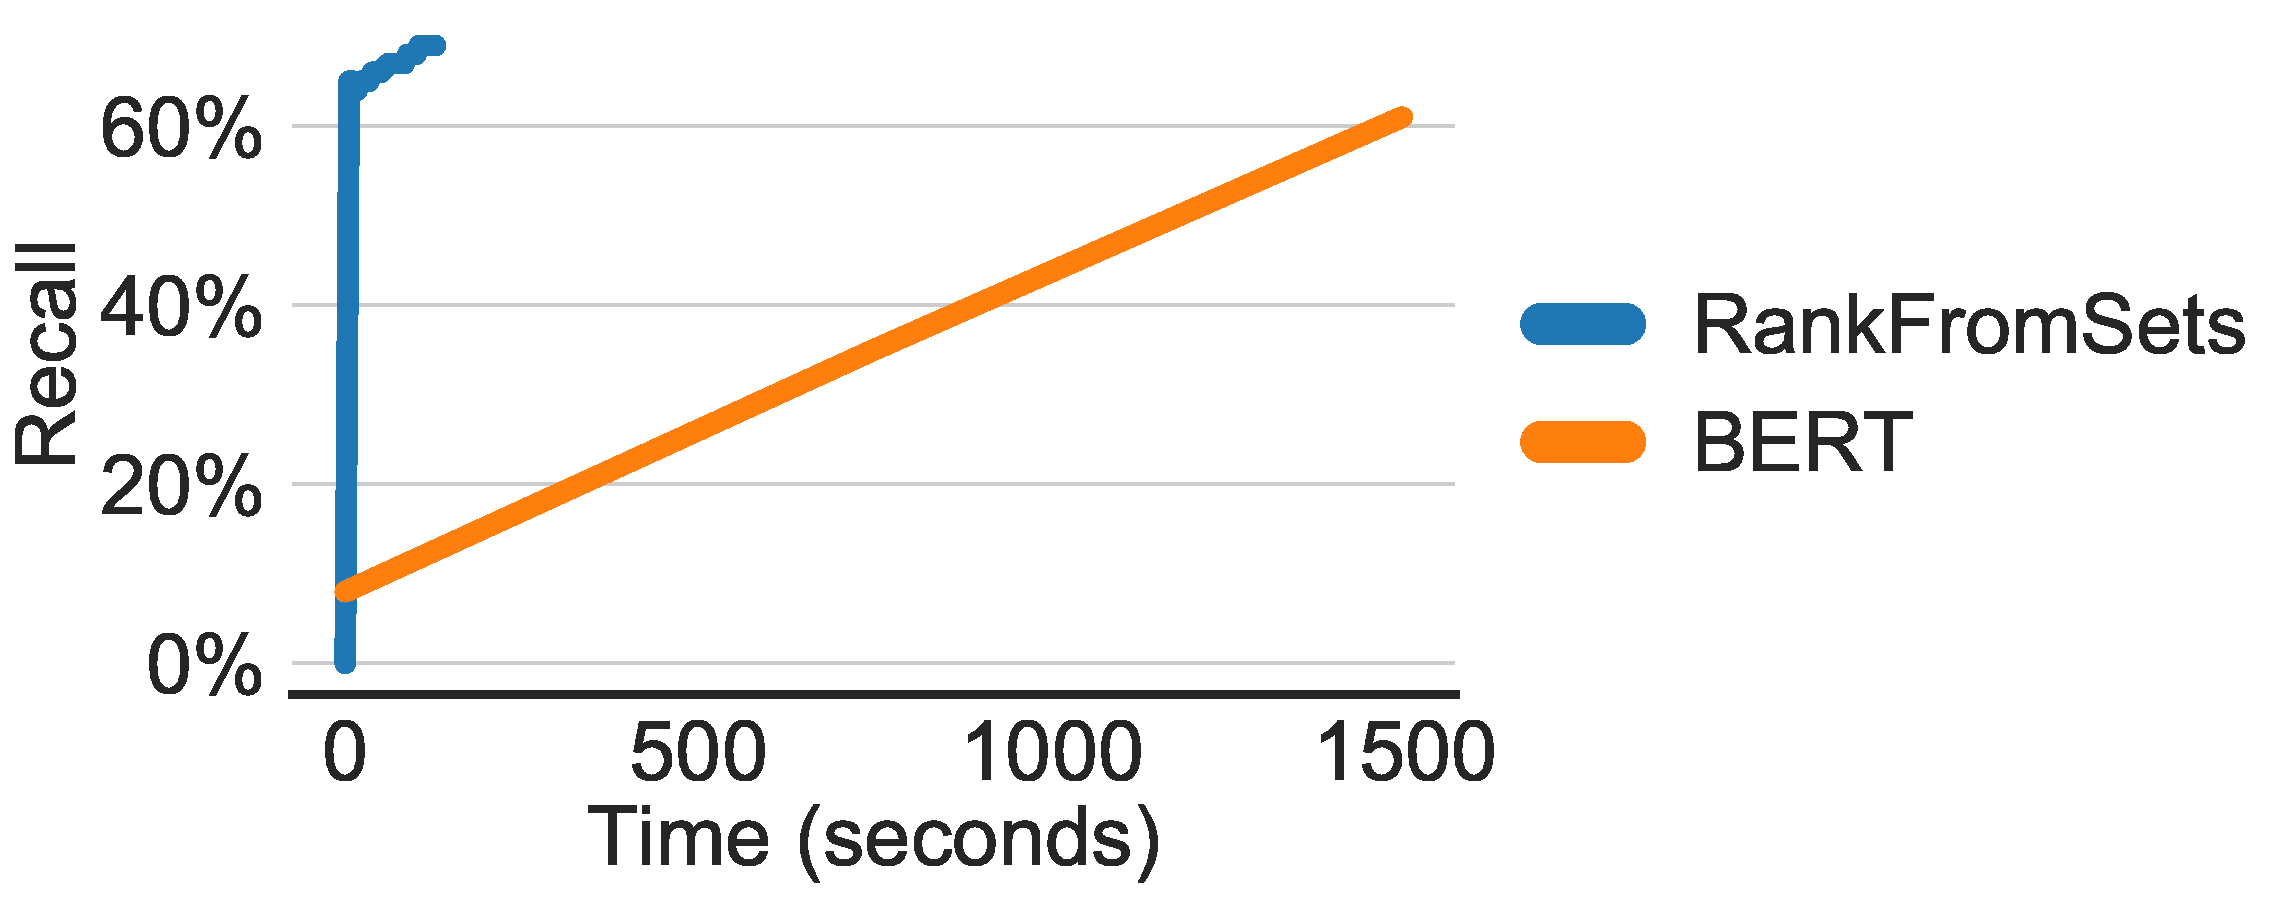
\includegraphics[width=0.95\linewidth]{fig/training-recall}
  \caption{\acrlong{rfs} outperforms models based on word embeddings
    permutation-marginalized recurrent neural networks (denoted by LSTM) on meal
    recommendation. The recommendation models are trained on data from a food
    tracking app as described in \Cref{sec:experiments_meals} and are evaluated
    using the sampled recall metric, \Cref{eq:sampled-recall}. The inner
    product, neural network, and residual regression functions for \acrlong{rfs}
    are in \Cref{eqn:rankfromsets,eqn:neural-network,eqn:residual}.}
  \label{fig:training-recall}
\end{figure}
% !TEX root = ../recommending-interesting-writing.tex
\begin{table}[tb]
\centering
\begin{tabular}{lSS}
\toprule
Recommendation Model & \multicolumn{1}{c}{Recall @ 1000 (\%)}
\\
\midrule
\acrlong{rfs} &  \bfseries 53.1\\
\acrshort{bert} & 46.6 \\
\bottomrule
\end{tabular}
% BERT 466/1000
% rankfromsets 531/1000
% \vspace{1ex}
\caption{\gls{rfs} outperforms \acrshort{bert} in an offline evaluation, on a task of predicting which articles editors at The Browser would feature based on words in the articles.}
\label{tab:recall}
\end{table}

\paragraph{Evaluation.} Qualitatively, editors at The Browser preferred the recommendations of our pipeline over their current workflow of a reading list sorted in terms of recency and use the system in production.
% !TEX root = set_recommendation.tex
\section{Discussion}

The task of recommending items with attributes is difficult for several reasons.
It is unclear how to incorporate set-valued side information into models that
scale to large numbers of items and attributes. In addition, existing
recommendation models that leverage item attributes are not directly tied to
evaluation metrics. We developed \acrlong{rfs}, a scalable recommendation model
for items with attributes. Theoretically, we showed that optimizing its loss
function optimizes recall, and that it can approximate a class of recommendation
models including content-based matrix factorization. Empirically, \gls{rfs}
outperformed competitors and scaled to large datasets.

\paragraph{Simple theory and implementation} It is surprising that \gls{rfs}
outperforms the collaborative topic Poisson factorization model in
\citet{gopalan2014content-based}, as \gls{rfs} is a much simpler model.
\gls{rfs} does not require approximate posterior inference as in \gls{ctpf}, but
mere binary classification. \gls{rfs} is also simpler in terms of
implementation: a scalable example is a few dozen lines of python in
\Cref{sec:code}, compared to several thousand lines of C++ released by the
authors of \gls{ctpf}.

\paragraph{Architectures} There is a wealth of deep learning models that can be
used to parameterize \gls{rfs}. For example, attention-based transformer
networks can operate on set-valued input~\cite{lee2018set-transformer} and are
an interesting choice of architecture for \gls{rfs}.
% larger batch sizes on cpu
% For good performance on the arXiv dataset, large batch sizes were necessary. We
% were limited in batch size due to our use of a GPU. Reimplementing the model in
% C++ would free the model from GPU memory restrictions, enabling larger batch
% sizes and better performance.
% optimization: ctpf benefits from coordinate ascent
% \paragraph{Optimization} Collaborative topic Poisson factorization as the latter
% enjoys an efficient optimization algorithm. The conjugacy properties of the
% matrix factorization model permit coordinate ascent and fast convergence in few
% iterations. The nonconvex objective function that \gls{rfs} relies on may be
% amenable to certain optimization techniques, such as dual coordinate
% ascent~\citep{yu2011dual}, and we leave this to future work.

\paragraph{Side information} The \gls{rfs} model can easily accommodate various
metadata about users, items, or attributes. Attribute-level or user-level side
information is particularly interesting, and when available, should lead to
improved recommendation performance.

% we did not study regularization
\paragraph{Regularization} Further performance gains from regularizing \gls{rfs}
are also interesting avenues for future work. L2 regularization for sparsity and
dropout for decorrelation may yield improvements.

% RMSProp~\cite{graves2013generating} was also tested when fitting
% \gls{rfs} to the arXiv data. This optimizer outperformed
% collaborative topic Poisson factorization in terms of both in-matrix precision
% and recall, but matched the performance of the matrix factorization model in
% terms of out-matrix precision and recall. This means there are tradeoffs of
% using different optimizers that depend on the data and evaluation metrics of
% interest.
% initializing to word2vec
\paragraph{Pretrained embeddings} We note that the word embedding baseline
performed slightly worse as collaborative topic Poisson factorization, which is
surprising given that the word embedding model is much simpler. Further
performance gains in \gls{rfs} should be possible by initializing user and item
attribute embeddings to pretrained word embeddings as in \citet{chen2017joint}.

% gap in prop 2
\paragraph{Theory (approximation)} \Cref{prop:universal-approximation} means
that \gls{rfs} can approximate the output of any order-invariant model
such as matrix factorization. However, there is no guarantee that fit with
maximum likelihood estimation using the objective in \Cref{eq:objective},
\gls{rfs} \emph{will} approximate a specific model. We leave the development of
such approximation techniques to future work.
% out-of-vocabulary words
% An open question is how to account for new attributes, for example in
% crowdsourced data. An extension of this work would be to combine it with
% character-level embeddings as in \cite{bojanowski2017enriching} to enable the
% model to better perform recommendations for out-of-vocabulary attributes.
% can we optimize metrics other than recall?
\paragraph{Theory (ranking metrics)} How well does binary classification perform
for other ranking-based recommendation metrics, such as non-discounted
cumulative gain? Analyzing this question is more difficult, and we leave this to
future work. We conjecture that a different loss function should allow a similar
proof to \Cref{prop:maximizing-recall}.

\paragraph{Theory of generalization} With sufficient data, \acrlong{rfs} can
learn arbitrary distributions of users consuming items with attributes. But
performance on finite data can vary. Developing generalization theory for
\acrlong{rfs} remains an open question.

% \section*{Acknowledgments}
% % and emotional support
% J.A. is grateful to Mark Goldstein and Bharat Srikisan for helpful
% discussions, and to Kyle Cranmer
% and the Center for Data Science at New York University for desk space. The
% experiments presented in this article were performed on computational resources
% supported by the Princeton Institute for Computational Science and Engineering
% and the Office of Information Technology's High Performance Computing Center and
% Visualization Laboratory at Princeton University.

%%% Local Variables:
%%% mode: latex
%%% TeX-master: "set_recommendation"
%%% End:
\section*{Acknowledgments}
The authors are grateful to Christian Bjartli for help with data collection.
\bibliographystyle{ACM-Reference-Format}
\bibliography{bib}
\end{document}